% !TeX program = xelatex
% 网络编程大作业报告 —— 用 XeLaTeX 编译：./build.sh
\documentclass[11pt,a4paper,fontset=fandol]{ctexart}

\usepackage{geometry}
\geometry{left=2.2cm,right=2.2cm,top=2.2cm,bottom=2.2cm}
\usepackage{booktabs}
\usepackage{tabularx}
\usepackage{longtable}
\usepackage{array}
\usepackage{multirow}
\usepackage{graphicx}
\usepackage{float}
\usepackage{xcolor}
\usepackage{listings}
\usepackage{caption}
\usepackage{enumitem}
\usepackage{fancyhdr}
\usepackage{tikz}
\usetikzlibrary{positioning,arrows.meta,calc}
\usepackage{hyperref}

\hypersetup{colorlinks=true,linkcolor=blue!45!black,urlcolor=blue!55!black}

\pagestyle{fancy}
\fancyhf{}
\fancyhead[L]{\small 网络编程大作业：带有文件传输功能的多播聊天工具}
\fancyhead[R]{\small\thepage}
\renewcommand{\headrulewidth}{0.4pt}
\setlength{\parskip}{2pt}
\emergencystretch=1.5em  % 中英混排断行缓冲

\lstset{
  basicstyle=\ttfamily\footnotesize,
  keywordstyle=\color{blue!70!black},
  commentstyle=\color{green!40!black},
  stringstyle=\color{red!55!black},
  frame=single,
  rulecolor=\color{gray!60},
  breaklines=true,
  columns=fullflexible,
  keepspaces=true,
  showstringspaces=false,
  tabsize=4,
  captionpos=b,
  aboveskip=6pt,
  belowskip=4pt,
}

\begin{document}

\begin{center}
{\LARGE\bfseries 网络编程大作业报告}\\[6pt]
{\large 带有文件传输功能的多播聊天工具}
\end{center}

\vspace{-0.3cm}
\begin{center}
\begin{tabular}{ll@{\hspace{2.2cm}}ll}
姓名：郑佳诚 & & 学号：57124434 & \\
\end{tabular}
\end{center}

\section{实验目的与要求}

设计并实现一个基于 UDP \textbf{多播}的 1-N 聊天工具（硬性要求：必须用多播实现，
做成服务器聊天室不合格），并满足：

\begin{enumerate}[itemsep=1pt,topsep=2pt]
  \item \textbf{(a) 文本传输}：聊天文字以多播报文在组内广播；
  \item \textbf{(b) 文件传输}：源通过多播把文件（音视频）发给多个接收方，接收方收到后能播放；
  \item \textbf{(c) 成员管理}：显示当前多播组成员、删除（踢出）成员等；
  \item \textbf{(d) 加密（加分）}：利用非对称密钥进行加密传输。
\end{enumerate}

\section{实验环境}

\begin{table}[H]
\centering\small
\begin{tabularx}{0.95\textwidth}{lX}
\toprule
项目 & 内容 \\
\midrule
操作系统 & Windows 11（另在 VirtualBox 虚拟机上做跨机验证） \\
语言/编译器 & C++17/20，MinGW-w64 g++ 15.2（\texttt{-O2 -Wall -Wextra} 零警告，静态链接，零第三方依赖） \\
网络 & Winsock2 UDP 多播，组地址 \texttt{239.255.42.99:54321} \\
加密 & Windows CNG（\texttt{bcrypt}）：RSA-2048、AES-256-GCM、SHA-256 \\
界面 & Win32 API 原生控件 \\
抓包 & Wireshark/tshark（VirtualBox Host-Only 出接口） \\
报告编译 & TeX Live 2025，XeLaTeX + ctex \\
\bottomrule
\end{tabularx}
\end{table}

\section{实验原理}

\subsection{IP 多播与组成员管理}

IP 多播使用 D 类地址（224.0.0.0--239.255.255.255）。其中 239.0.0.0/8 为"本地组织
范围"，路由器默认不向组织外转发，适合局域网内的组通信，本系统即选用
\texttt{239.255.42.99}。发送方把 UDP 数据报的目的地址填成组地址即可，交换机与
路由器把它"一次分发、多处接收"，与逐一单播 $N$ 份相比，发送方带宽恒为一份。

多播地址只到 IP 层为止。以太网帧的接收依据是 48 位 MAC 地址，多播 IP 地址的低
23 位直接填进 \texttt{01:00:5e:xx:xx:xx} 的对应位——IP 组地址有 28 位有效信息而 MAC
只容纳 23 位，因此\textbf{平均每 32 个多播组共享一个 MAC 地址}。网卡按 MAC 过滤后，
内核还必须再按目的 IP 过滤一次，才能把"恰好同 MAC"的无关组流量丢掉；这也解释了
为什么内核要维护一张"哪些套接字加入了哪些组"的成员表——它正是本系统单机演示
可行性的基础（见 \S\ref{sec:loop}）。

应用通过 \texttt{setsockopt(IP\_ADD\_MEMBERSHIP)} 加入组，内核随即在该网卡上发送
IGMP 成员关系报告，路由器据此决定是否向本网段转发该组流量；组地址选 \texttt{239/8}
与 \texttt{IP\_MULTICAST\_TTL=1} 共同把传播范围约束在一个局域网内。

\begin{table}[H]
\centering\footnotesize
\begin{tabularx}{0.98\textwidth}{lXXX}
\toprule
 & 广播 & 中心服务器转发 & \textbf{多播（本方案）} \\
\midrule
发送方开销 & 一份，全网强制接收 & $N$ 份逐个单播 & \textbf{一份，仅订阅者收} \\
服务器 & 无 & 必须部署，是单点 & \textbf{无（对等）} \\
跨网段 & 泛洪全网 & 依赖服务器位置 & 需路由器开多播路由，TTL 可控 \\
成员控制 & 无 & 服务器维护 & 应用层自建（本作业核心之一） \\
\bottomrule
\end{tabularx}
\caption{三种 1-N 通信方式的对比：题目要求且本系统全部功能只依赖多播}
\label{tab:mc-cmp}
\end{table}

\subsection{为什么单机即可完成实验：回环与端口复用}
\label{sec:loop}

多播回环（\texttt{IP\_MULTICAST\_LOOP=ON}）开启后，IP 层把发出的多播包在送出网卡
的同时\textbf{额外回送一份到本机协议栈}；内核查询成员表，把副本投递给本机每一个
加入了该组、且绑定在该端口的套接字。配合 \texttt{SO\_REUSEADDR} 允许多个套接字
绑定同一端口，一台主机上就能跑起任意多个"虚拟成员"。

\begin{figure}[H]
\centering
\begin{tikzpicture}[font=\small,
  inst/.style={draw=black!55, rounded corners=2pt, inner sep=4pt, align=center},
  kernel/.style={draw=black!55, fill=gray!10, rounded corners=2pt, inner sep=5pt, align=center}]
  \node[inst] (a) at (0,0)   {实例 A\\ UUID-A / 密钥 A};
  \node[inst] (b) at (4.2,0) {实例 B\\ UUID-B / 密钥 B};
  \node[inst] (c) at (8.4,0) {实例 C\\ UUID-C / 密钥 C};
  \node[kernel, minimum width=10.6cm, below=9mm of b] (k) {\textbf{Windows 协议栈}：按组成员表分发副本\\ 每个加入组且绑定该端口的套接字各得一份};
  \draw[-Latex, thick]  (a.south) -- (a.south |- k.north);
  \draw[-Latex, thick]  (b.south) -- (b.south |- k.north);
  \draw[-Latex, thick]  (c.south) -- (c.south |- k.north);
  \draw[-Latex, thick, dashed] ([xshift=5mm]k.north -| a.south) -- ([xshift=5mm]a.south);
  \draw[-Latex, thick, dashed] ([xshift=5mm]k.north -| b.south) -- ([xshift=5mm]b.south);
  \draw[-Latex, thick, dashed] ([xshift=5mm]k.north -| c.south) -- ([xshift=5mm]c.south);
  \node[font=\scriptsize, gray, below=1.2mm of k, align=center, text width=11cm]
    {实线：sendto 组地址（TTL=1）；虚线：LOOP=ON 的回环副本，投递给本机全部成员套接字\\
     （含发送者自己一份，应用层按 UUID 丢弃，避免重复显示）};
\end{tikzpicture}
\caption{单机多实例的等价性：实例间零共享状态，仅通过内核回环的多播报文同步}
\label{fig:loop}
\end{figure}

\noindent 这种等价性是\textbf{逻辑上的}而非模拟：三个实例是三个独立进程，各有
UUID 身份、RSA 密钥与成员表，除了多播报文没有任何共享内存或 IPC，应用层无法
区分"包从回环来"还是"包从网卡来"。专门的 \texttt{nettest} 自测让同机两个多播
套接字互发，双方各收全 10/10 个探测包，证实了这条路径的可达性与"逐套接字分发"
的语义。跨机部署（\S\ref{sec:result}）的结果与单机一致，进一步印证了这一点。

\subsection{UDP 多播的不可靠性与对策}

UDP 多播不提供任何可靠性：网络拥塞时交换机/路由器直接丢弃；接收主机套接字
缓冲区满时内核同样\textbf{静默丢包}（突发灌包正是缓冲区溢出的首因，所以发送端
必须限速）；而且没有任何重传机制。多播的"一次发送"意味着\textbf{一个丢包同时
影响全体接收者}。因此文件传输必须自己补可靠性，业界有三类做法：

\begin{table}[H]
\centering\footnotesize
\begin{tabularx}{0.98\textwidth}{lXX}
\toprule
方案 & 原理 & 取舍 \\
\midrule
ACK 确认 & 每包等全体确认 & $N$ 个接收方产生 ACK 风暴，发送端状态重 \\
FEC 前向纠错 & 冗余修复包 & 编解码开销，修复能力有上限，实现复杂 \\
\textbf{NACK 选择重传} & 接收方发现缺失才请求 & \textbf{本方案}：仅缺失者发声，配合区间编码压缩请求 \\
\bottomrule
\end{tabularx}
\caption{可靠多播的三类对策}
\label{tab:rel}
\end{table}

\noindent 本系统选择 NACK：接收方按位图自查缺失，把缺失块压缩成
$[start,end]$ \textbf{区间列表}请求重传——普通丢包只有零星小区间，晚加入者缺失
上万块也只占一两个区间；发送端聚合所有接收方的请求后只补缺失块。为抑制 NACK
风暴，接收端按自身节拍评估（收到 END 后 800\,ms 复查、发出 NACK 后 2.5\,s 再查）
而非对每个丢包立即反应；发送端以 2\,s 窗口聚合请求后统一补发。

\section{系统设计}

\subsection{总体架构：无服务器的对等多播}

系统\textbf{不设任何中心服务器}，唯一的通信设施是一个 UDP 多播组：每个实例启动后
创建 UDP 套接字、绑定 54321 端口并 \texttt{IP\_ADD\_MEMBERSHIP} 加入组，此后聊天、
文件块、心跳、踢人、密钥分发等\textbf{所有}报文都只发往组地址——发一次，组内全员
各收一份，天然满足 1-N。多播组的成员关系在 IP/IGMP 层，应用查不到，因此成员表由
应用层自行维护（见 \S\ref{sec:member}）。

\begin{figure}[H]
\centering
\begin{tikzpicture}[
  box/.style={draw=black!55, rounded corners=2pt, align=center, inner sep=5pt, minimum height=8mm},
  lab/.style={font=\footnotesize\bfseries, anchor=west},
  arr/.style={Latex-Latex, thick, black!60}]
  \node[box, fill=blue!8,  text width=10.6cm] (ui)   {\textbf{UI 层}（Win32 单线程消息循环）：聊天区 · 成员列表 · 加密开关 · 进度条};
  \node[box, fill=green!8, text width=10.6cm, below=4mm of ui]   (core) {\textbf{应用层}：MemberManager（成员表/踢人） · FileXfer（文件收发） · ChatCtrl};
  \node[box, fill=orange!10, text width=10.6cm, below=4mm of core] (sec) {\textbf{crypto 层}：RSA-2048（信封/签名） · AES-256-GCM · 组密钥分发};
  \node[box, fill=red!8,   text width=10.6cm, below=4mm of sec]  (net)  {\textbf{protocol/net 层}：32B 二进制头 + TLV 载荷（大端） · MulticastSocket + 接收线程};
  \node[below=6mm of net, font=\small\bfseries] (group) {UDP 多播组 239.255.42.99:54321};
  \draw[arr] (ui)   -- (core);
  \draw[arr] (core) -- (sec);
  \draw[arr] (sec)  -- (net);
  \draw[arr] (net)  -- (group);
  \node[lab, right=2mm of ui, text width=3.4cm, font=\footnotesize] {接收线程把报文 \texttt{PostMessage} 给 UI 线程，UI 更新免锁};
  \node[lab, right=2mm of net, text width=3.4cm, font=\footnotesize] {文件发送走独立节拍线程（500 包/秒）};
\end{tikzpicture}
\caption{系统分层架构（除 UI 外，层间仅通过报文与明确接口交互）}
\label{fig:arch}
\end{figure}

线程模型：主线程跑 Win32 消息循环；接收线程阻塞轮询多播报文，整包拷贝后
\texttt{PostMessage} 投递给主线程，所有状态变更集中在 UI 线程，天然免锁；
文件发送用独立线程按节拍发包；1\,s 周期定时器驱动心跳、超时扫描与进度刷新。

\subsection{源码结构}

\begin{lstlisting}[caption={源码结构（mcast-chat/，约 4600 行 C++，零第三方依赖）},label={lst:tree}]
src/
 |- main.cpp            入口：命令行、启动顺序（身份 -> 密钥 -> 窗口 -> 接收线程）、消息循环
 |- app.hpp/.cpp        全局 App：昵称 / UUID / 发送序号 / 套接字 / 测试钩子
 |- net/                MulticastSocket（加组/TTL/回环/端口复用）+ 接收线程（PostMessage 投递）
 |- protocol/           32B 二进制头 + 大端序列化 Writer/Reader + 各消息编解码
 |- core/               MemberManager（成员表/踢人） FileXfer（文件收发） ChatCtrl（聊天）
 |- crypto/             CNG 封装：RSA-2048 / AES-256-GCM / SHA-256 / SecureSession（组密钥）
 |- ui/                 Win32 主窗口：聊天区 / 成员列表 / 加密开关 / 进度条 / 右键菜单
 `- util/               UTF-8 <-> UTF-16 转换、exe 目录定位、调试日志
\end{lstlisting}

\noindent 分层间只通过报文与明确接口交互：UI 不直接碰套接字，crypto 不认识 UI。
Windows 程序的 UI 必须单线程（消息循环），因此网络接收放在独立线程并以
\texttt{PostMessage} 把整包投递回 UI 线程处理（片段~\ref{lst:rx}）——投递的是堆上
拷贝，由 UI 线程释放，跨线程不共享任何可变结构，全程序不需要一把锁（组密钥除外，
它会被发送线程读取，用互斥量保护）。

\begin{lstlisting}[caption={net/rx\_thread.cpp：接收线程把整包投递给 UI 线程},label={lst:rx}]
static DWORD WINAPI rx_thread_proc(LPVOID) {
    App& a = app();
    std::vector<uint8_t> buf(65536);
    while (!a.rxStop.load()) {
        uint32_t fromIp = 0;
        int n = a.sock.recv(buf.data(), buf.size(), &fromIp);   /* 300ms 超时轮询 */
        if (n <= 0) continue;                    /* 超时：回去检查退出标志 */
        if (n < (int)proto::kHeaderSize) continue;
        RxPacket* pkt = malloc 包头 + n;         /* 堆上拷贝，跨线程所有权转移 */
        pkt->fromIp = fromIp; pkt->len = n;
        memcpy(pkt->data, buf.data(), n);
        if (!PostMessageW(a.hwnd, WM_APP_RX, 0, (LPARAM)pkt)) free(pkt);
    }
    return 0;
}
\end{lstlisting}

\subsection{报文协议}

自定义二进制协议：32 字节定长头 + 载荷，全部网络字节序，单报文 $\le$1400\,B
（以太网 MTU 内，避免 IP 分片放大丢包）。序列化用手写的
\texttt{put\_u16/u32/utf8} 系列，不做 struct 裸拷贝，避开填充与字节序陷阱。

\begin{table}[H]
\centering\small
\begin{tabularx}{0.95\textwidth}{clcl}
\toprule
偏移 & 大小 & 字段 & 说明 \\
\midrule
0 & 4 & magic & \texttt{'MCHT'} \\
4 & 1 & version & 协议版本（1） \\
5 & 1 & type & 消息类型（见表~\ref{tab:types}） \\
6 & 2 & flags & bit0=载荷已加密（AES-GCM），bit1=附 RSA-PSS 签名 \\
8 & 16 & senderId & 成员 UUID（身份标识与自环过滤） \\
24 & 4 & seq & 发送端单调递增序号（排序/防重放） \\
28 & 4 & payloadLen & 载荷长度 \\
32 & $\dots$ & 载荷 & 按类型解析 \\
\bottomrule
\end{tabularx}
\caption{报文定长头}
\label{tab:hdr}
\end{table}

\begin{table}[H]
\centering\footnotesize
\begin{tabularx}{0.98\textwidth}{llX}
\toprule
类别 & type & 用途与载荷要点 \\
\midrule
\multirow{6}{*}{控制面} & HELLO / HELLO\_ACK & 入组宣告/应答：昵称 + joinTime + RSA 公钥（握手建表） \\
 & HEARTBEAT & 3\,s 一次保活，载荷自带昵称与 joinTime（丢包自愈） \\
 & BYE & 正常退组，立即从各成员表移除 \\
 & KICK & 房主踢人：targetId + 房主 RSA-PSS 签名，全员验签 \\
 & KEY\_DIST & 组密钥信封分发：keyId + \{成员 $\to$ RSA-OAEP(组密钥)\} \\
\midrule
\multirow{5}{*}{数据面} & TEXT & 昵称 + 正文；恒附 RSA-PSS 签名 \\
 & FILE\_META / DATA / END & 文件元组（名称/大小/SHA-256/分块数）、1024\,B 分块、发完通告 \\
 & NACK & 缺失区间列表（$[start,end]$ 对），请求重传 \\
 & FILE\_CANCEL & 发送方放弃 \\
\bottomrule
\end{tabularx}
\caption{消息类型（控制面明文传输；数据面可加密）}
\label{tab:types}
\end{table}

\noindent 两个代表性载荷格式。FILE\_DATA（未加密时）与 KEY\_DIST：

\begin{lstlisting}[caption={数据面与密钥分发的载荷布局}]
FILE_DATA:  [ fileId(16B) | chunkSeq(4B) | data(<=1024B) ]
KEY_DIST :  [ keyId(4B) | count(4B) | ( targetId(16B) | len(2B) | RSA-OAEP(组密钥,256B) ) * count ]
            开启加密后数据面整体再被 AES-GCM 加密：payload = [ keyId(4B) | 密文+tag(16B) ]
            两个 keyId 含义不同：前者是 KEY_DIST 里"给谁的信封"，后者是"本包用第几把组密钥"
\end{lstlisting}

\section{关键实现}

\subsection{多播通信与单机演示原理}

多播套接字的关键配置只有四条（片段~\ref{lst:mc}）：绑定端口前开
\texttt{SO\_REUSEADDR}（允许多实例共存）、加入组 \texttt{IP\_ADD\_MEMBERSHIP}、
\texttt{IP\_MULTICAST\_TTL=1}（不出本地网段）、\texttt{IP\_MULTICAST\_LOOP=ON}。

\begin{lstlisting}[caption={net/multicast.cpp：多播套接字关键配置},label={lst:mc}]
BOOL reuse = TRUE;   /* 允许同机多实例绑定同一端口 —— 单机演示 1-N 的关键之一 */
setsockopt(sock_, SOL_SOCKET, SO_REUSEADDR, (const char*)&reuse, sizeof(reuse));
ip_mreq mreq{};      /* 加入多播组 */
mreq.imr_multiaddr = dst_.sin_addr;
mreq.imr_interface.s_addr = htonl(INADDR_ANY);
setsockopt(sock_, IPPROTO_IP, IP_ADD_MEMBERSHIP, (const char*)&mreq, sizeof(mreq));
u_char ttl = 1;      /* 同网段 */
setsockopt(sock_, IPPROTO_IP, IP_MULTICAST_TTL, (const char*)&ttl, sizeof(ttl));
BOOL loop = TRUE;    /* 本机回环：单机开多实例演示 1-N 的关键之二 */
setsockopt(sock_, IPPROTO_IP, IP_MULTICAST_LOOP, (const char*)&loop, sizeof(loop));
\end{lstlisting}

\noindent \textbf{单机即可完成实验的原因}：多播回环开启后，IP 层把发出的多播包
额外回送一份到本机协议栈；内核按"本机哪些套接字加入了该组"逐个投递副本，配合
端口复用，本机多个实例在网络上完全等价于多台机器接在同一交换机下。三个实例是
三个独立进程，各有自己的 UUID 身份、RSA 密钥对、成员表、收发线程——它们之间除了
多播包**没有任何共享内存或 IPC**，所以应用层逻辑与跨机器完全一致（跨机验证见 \S\ref{sec:result}）。
区别仅在于回环路径几乎不丢包，所以代码还内置 \texttt{-{}-drop N} 测试钩子，
在接收端人为丢弃每第 $N$ 块，验证可靠性机制真实生效（见 \S\ref{sec:auto}）。

\subsection{成员管理（要求 c）}
\label{sec:member}

多播成员关系在 IP 层不可查询，成员表必须在应用层自建：

\begin{enumerate}[itemsep=1pt,topsep=2pt]
  \item \textbf{建表}：新成员多播 HELLO（昵称+joinTime+RSA 公钥），在线成员入表并回
        HELLO\_ACK，新成员据此建立全表；HELLO 连发 3 次抗丢包；
  \item \textbf{保活与三级删除}：每 3\,s 广播心跳（自带身份信息，任何报文都能自愈
        成员表）；10\,s 无心跳标记离线、20\,s 自动移除；正常退出在窗口销毁钩子里发
        BYE 立即移除；房主可踢人（见下）；
  \item \textbf{房主}：joinTime 最早（系统时钟毫秒，跨机可比）且在线者担任，
        离线自动继任；踢人报文须来自当前房主并附其 RSA 签名；
  \item \textbf{踢人}：房主多播 KICK（targetId + RSA-PSS 签名），全员验签后把目标
        移出成员表并加入黑名单（忽略其一切后续报文）；被踢端收到验签通过的 KICK
        后禁用输入、3\,s 后自动退出。
\end{enumerate}

\noindent 心跳、超时与房主选举都收敛在同一个 1\,s 节拍函数里（片段~\ref{lst:tick}）：
超时阈值是心跳周期的三倍以上（10\,s/20\,s），避免单次丢包误判；房主定义为
"joinTime 最早且在线"，joinTime 取系统时钟毫秒（跨机可比，同毫秒按 UUID 决胜），
成员增删后重算，房主离线自然由次早者继任。

\begin{figure}[H]
\centering
\begin{tikzpicture}[font=\scriptsize,
  lane/.style={draw=black!55, thick},
  msg/.style={-{Latex}, thick},
  note/.style={font=\scriptsize, gray}]
  \def\Xa{0} \def\Xb{4.2} \def\Xc{8.4}
  \node[draw, rounded corners=2pt, fill=blue!8]   (ha) at (\Xa,0) {新成员 X};
  \node[draw, rounded corners=2pt, fill=green!8]  (hb) at (\Xb,0) {房主 A};
  \node[draw, rounded corners=2pt, fill=green!8]  (hc) at (\Xc,0) {在线成员 B};
  \draw[lane] (ha.south) -- ++(0,-6.4);
  \draw[lane] (hb.south) -- ++(0,-6.4);
  \draw[lane] (hc.south) -- ++(0,-6.4);
  \draw[msg] (\Xa,-0.7) -- node[above]{HELLO（昵称+joinTime+公钥，连发3次）} (\Xb,-0.7);
  \draw[msg] (\Xa,-0.7) -- (\Xc,-0.7);
  \draw[msg] (\Xb,-1.4) -- node[above]{HELLO\_ACK（自己的身份+公钥）} (\Xa,-1.4);
  \draw[msg] (\Xc,-1.9) -- node[above]{HELLO\_ACK} (\Xa,-1.9);
  \node[note] at (5.4,-2.5) {X 建立全表，全员把 X 入表并触发组密钥重分发};
  \draw[msg, dashed] (\Xa,-3.1) -- node[above]{HEARTBEAT（3s 一次，全体广播）} (\Xb,-3.1);
  \node[note] at (5.0,-3.7) {…… X 所在进程崩溃，心跳停止 ……};
  \draw[msg, dotted] (\Xb,-4.4) -- node[above]{10s 无心跳：标记离线} (\Xc,-4.4);
  \draw[msg, dotted] (\Xb,-5.0) -- node[above]{20s：从成员表移除} (\Xc,-5.0);
  \node[note] at (5.0,-5.6) {（若房主主动踢人：KICK 携带房主 RSA 签名，全员验签后移除并加黑名单）};
  \draw[msg] (\Xb,-6.2) -- node[above]{重算房主：joinTime 次早者继任} (\Xc,-6.2);
\end{tikzpicture}
\caption{成员管理报文时序：握手建表、心跳保活、超时删除与房主继任}
\label{fig:seq-member}
\end{figure}

\begin{lstlisting}[caption={core/member\_mgr.cpp：1s 节拍里的心跳与超时扫描},label={lst:tick}]
void MemberManager::tick() {
    ++tickCount_;
    if (helloSends_ > 0) { send_hello(); --helloSends_; }   /* 入组 HELLO 补发 */
    if (tickCount_ % 3 == 0) send_heartbeat();              /* 3s 心跳 */
    const uint64_t now = now_tick();
    for (size_t i = 0; i < list_.size();) {
        Member& m = list_[i];
        if (m.self) { ++i; continue; }
        uint64_t idle = now - m.lastSeen;
        if (m.online && idle > 10000) {                     /* 10s 无心跳 -> 离线 */
            m.online = false;
            events_.push_back({MemberEvent::Offline, m.name});
        } else if (!m.online && idle > 20000) {             /* 20s -> 移除 */
            events_.push_back({MemberEvent::Left, m.name});
            list_.erase(list_.begin() + i);
            continue;
        }
        ++i;
    }
    recompute_host();                                       /* 房主可能变化 */
}
\end{lstlisting}

\subsection{文件的可靠多播传输（要求 b）}

UDP 多播不可靠，可靠性自己补，方案为"分块 + 节拍 + 位图 + NACK 选择重传"：

\begin{enumerate}[itemsep=1pt,topsep=2pt]
  \item 发送：文件按 1024\,B 分块，专用线程以 500 包/秒匀速多播（突发灌包是丢包
        首因）；META（含 SHA-256）开头连发 3 次且每 5\,s 重发，晚加入者可中途接入；
  \item 接收：按 META 建立位图与临时文件，收块置位落盘；收到 END 后 800\,ms 复查
        位图，缺失块以\textbf{区间}编码进 NACK（单包最多 160 个区间，2\,GB 文件全部
        缺失也只有 1 个区间），此后每 2.5\,s 自查重发；
  \item 重传：发送端按 2\,s 窗口收集各接收方的 NACK，只重传缺失块并重发 END；
        最多 5 轮，超限发 FILE\_CANCEL 放弃；接收 30\,s 无活动判超时；
  \item 完整性与落盘：收全后先写临时文件，SHA-256 校验一致才改名为
        \texttt{received\textbackslash 原名}（重名自动追加序号），目录\textbf{绝对路径}
        锚定在 exe 所在目录（文件对话框会改变进程工作目录，相对路径会让文件散落，
        这是开发中实际踩到并修复的坑）；完成后"播放"按钮调用系统默认播放器。
\end{enumerate}

\noindent 区间化 NACK 的核心是把位图扫描结果压缩成 $[start,end]$ 对
（片段~\ref{lst:ranges}）：普通丢包产生零星小区间，一两个报文就能装下；而晚加入者
缺失上万块也只是\textbf{一个}区间——编码长度只与"缺失段数"有关，与缺失总量无关。
整个收发流程的报文时序见图~\ref{fig:seq-file}。

\begin{lstlisting}[caption={core/file\_xfer.cpp：位图 -> 缺失区间列表},label={lst:ranges}]
std::vector<std::pair<uint32_t,uint32_t>>
missing_ranges(const std::vector<uint8_t>& bits, uint32_t total) {
    std::vector<std::pair<uint32_t,uint32_t>> out;
    uint32_t runStart = UINT32_MAX;
    for (uint32_t i = 0; i < total; ++i) {
        bool have = bits[i >> 3] & (1 << (i & 7));
        if (!have && runStart == UINT32_MAX) runStart = i;   /* 缺失段开始 */
        if ( have && runStart != UINT32_MAX) {               /* 缺失段结束 */
            out.push_back({runStart, i - 1});
            runStart = UINT32_MAX;
        }
    }
    if (runStart != UINT32_MAX) out.push_back({runStart, total - 1});
    return out;
}
\end{lstlisting}

\begin{figure}[H]
\centering
\begin{tikzpicture}[font=\scriptsize,
  lane/.style={draw=black!55, thick},
  msg/.style={-{Latex}, thick},
  note/.style={font=\scriptsize, gray}]
  \def\Xa{0} \def\Xb{4.2} \def\Xc{8.4}
  \node[draw, rounded corners=2pt, fill=blue!8]  (ha) at (\Xa,0) {发送方 S};
  \node[draw, rounded corners=2pt, fill=green!8] (hb) at (\Xb,0) {接收方 $R_1$};
  \node[draw, rounded corners=2pt, fill=green!8] (hc) at (\Xc,0) {接收方 $R_2$};
  \draw[lane] (ha.south) -- ++(0,-6.6);
  \draw[lane] (hb.south) -- ++(0,-6.6);
  \draw[lane] (hc.south) -- ++(0,-6.6);
  \draw[msg] (\Xa,-0.7) -- node[above]{FILE\_META（名称/大小/SHA-256/分块数，开头 3 次）} (\Xb,-0.7);
  \draw[msg] (\Xa,-0.7) -- (\Xc,-0.7);
  \draw[msg] (\Xa,-1.5) -- node[above]{FILE\_DATA（1024B/块，500 包/秒节拍，seq 递增）} (\Xb,-1.5);
  \draw[msg] (\Xa,-1.5) -- (\Xc,-1.5);
  \node[note] at (5.2,-2.2) {$R_1,R_2$：位图置位、写临时文件；期间每 5s 重发一次 META（晚加入者可接入）};
  \draw[msg] (\Xa,-2.9) -- node[above]{FILE\_END（首轮发完）} (\Xb,-2.9);
  \draw[msg] (\Xa,-2.9) -- (\Xc,-2.9);
  \node[note] at (5.2,-3.5) {+800ms：$R_1$ 缺 \{5,9\}，$R_2$ 缺 \{0--4\} -> 各自发 NACK（区间列表）};
  \draw[msg] (\Xb,-4.2) -- node[above]{NACK（缺失区间）} (\Xa,-4.2);
  \draw[msg] (\Xc,-4.7) -- node[below=1pt]{NACK（缺失区间）} (\Xa,-4.7);
  \draw[msg] (\Xa,-5.4) -- node[above]{只重传被请求的块 + FILE\_END（2s 窗口聚合，最多 5 轮）} (\Xb,-5.4);
  \draw[msg] (\Xa,-5.4) -- (\Xc,-5.4);
  \node[note] at (5.2,-6.0) {收全：SHA-256 校验 -> 改名入 received 目录；30s 无活动判超时放弃};
\end{tikzpicture}
\caption{文件传输报文时序：节拍多播、位图自查、区间 NACK 与选择重传}
\label{fig:seq-file}
\end{figure}

\subsection{非对称加密传输（要求 d）}

采用\textbf{信封方案}：非对称算法只负责身份认证与"发钥匙"，大流量载荷用对称算法
加密——这是密钥体系的标准姿势（RSA 直接加密大文件既慢又危险）。

\begin{enumerate}[itemsep=1pt,topsep=2pt]
  \item \textbf{身份}：每个成员启动时用 CNG 生成 RSA-2048 密钥对，公钥随 HELLO 广播；
  \item \textbf{组密钥分发}：房主生成 32\,B 组会话密钥，对每个在线成员的公钥做
        RSA-OAEP(SHA-256) 加密成"信封"，以 KEY\_DIST 多播（每包 4 个信封，超出分包）；
        各成员用自己的私钥解出组密钥；成员变化时去抖 2\,s 后自动重分发；
  \item \textbf{数据面加密}：TEXT/FILE\_*$^{}$载荷 = keyId(4\,B) + AES-256-GCM(密文+tag)。
        nonce 由 senderId 前 8\,B 与 seq 确定性派生（同一密钥下不重放、不占带宽）；
        AAD 绑定 senderId$\|$seq$\|$type，防止报文被裁剪、拼接或篡改；载荷带 keyId，
        重分发期间保留上一把密钥用于解在途旧包，文件发送线程持密钥快照，换钥不断传输；
  \item \textbf{签名}：TEXT 恒附 RSA-PSS 签名（flags bit1），KICK 由房主签名
        （覆盖 targetId$\|$senderId），验签失败一律丢弃；
  \item \textbf{强制离组}：被踢/退出成员被移出公钥表，不在新密钥的信封名单里——
        即便仍留在多播组，也解不开后续任何内容。
\end{enumerate}

\noindent 加密与解密收敛在 \texttt{seal\_payload}/\texttt{unseal} 两个函数里
（片段~\ref{lst:seal}）：发送侧统一决定加密与签名标志，接收侧按 flags 逆向还原。
nonce 不占用带宽——由 senderId 前 8 字节与包头里的 seq 拼成 12 字节（96 位），
同一密钥下同一 (sender, seq) 只会出现一次，从构造上杜绝重放；AAD 绑定包头三要素，
把密文"钉"在它所属的报文上，裁剪、拼接、改类型都会导致 GCM 校验失败。

\begin{lstlisting}[caption={crypto/secure\_session.cpp：统一加密封包与旧钥回退},label={lst:seal}]
std::string SecureSession::seal_payload(uint8_t type, const proto::Uuid& sender,
                                        uint32_t seq, const std::string& plain,
                                        uint16_t& flags, const KeySnapshot* keyOverride) {
    flags = 0;
    std::string body = plain;
    if (is_data_plane(type)) {                       /* TEXT 与 FILE_* 才加密 */
        KeySnapshot ks = keyOverride ? *keyOverride : current_key();
        if (enabled_ && !ks.key.empty()) {
            std::string ct = encrypt_with(ks, sender, seq, type, plain);
            if (!ct.empty()) {
                body = be32(ks.keyId) + ct;          /* 载荷前缀 keyId，供回退选钥 */
                flags |= FLAG_ENCRYPTED;
            }
        }
    }
    if (type == proto::MSG_CHAT_TEXT) {              /* TEXT 恒签名：防伪造发送者 */
        std::string sig;
        if (sign_data(plain, sig)) { body += sig; flags |= FLAG_SIGNED; }
    }
    return body;
}

std::string SecureSession::decrypt_with(uint32_t keyId, ...) const {
    std::string key;
    {   std::lock_guard<std::mutex> g(keyMtx_);
        if      (keyId == keyId_ && haveKey_) key = groupKey_;   /* 当前密钥 */
        else if (keyId == prevKeyId_)        key = prevKey_;     /* 换钥瞬间回退旧钥 */
        else return "";
    }   /* AES-256-GCM 解密 + tag 校验，失败即认为被篡改/密钥不符 */
    return aes256gcm_decrypt(key, nonce_from(sender, seq), aad, cipher);
}
\end{lstlisting}

\section{实验结果与分析}
\label{sec:result}

\subsection{跨机多播聊天与成员管理}

图~\ref{fig:members} 为四实例（ZhangSan/LiSi/WangWu/maluser）运行在 VirtualBox
Host-Only 网段（192.168.56.0/24）上的真实跨机部署：每个窗口的成员列表都完整列出
四名成员，本机显示"(本机)"、其余显示 192.168.56.1，昵称、状态、房主角色四处一致；
maluser（自称"恶意用户"）入组后同样被所有成员的成员表接纳，说明多播的 1-N 通告
与握手对"陌生成员"一视同仁。

\begin{figure}[H]
\centering
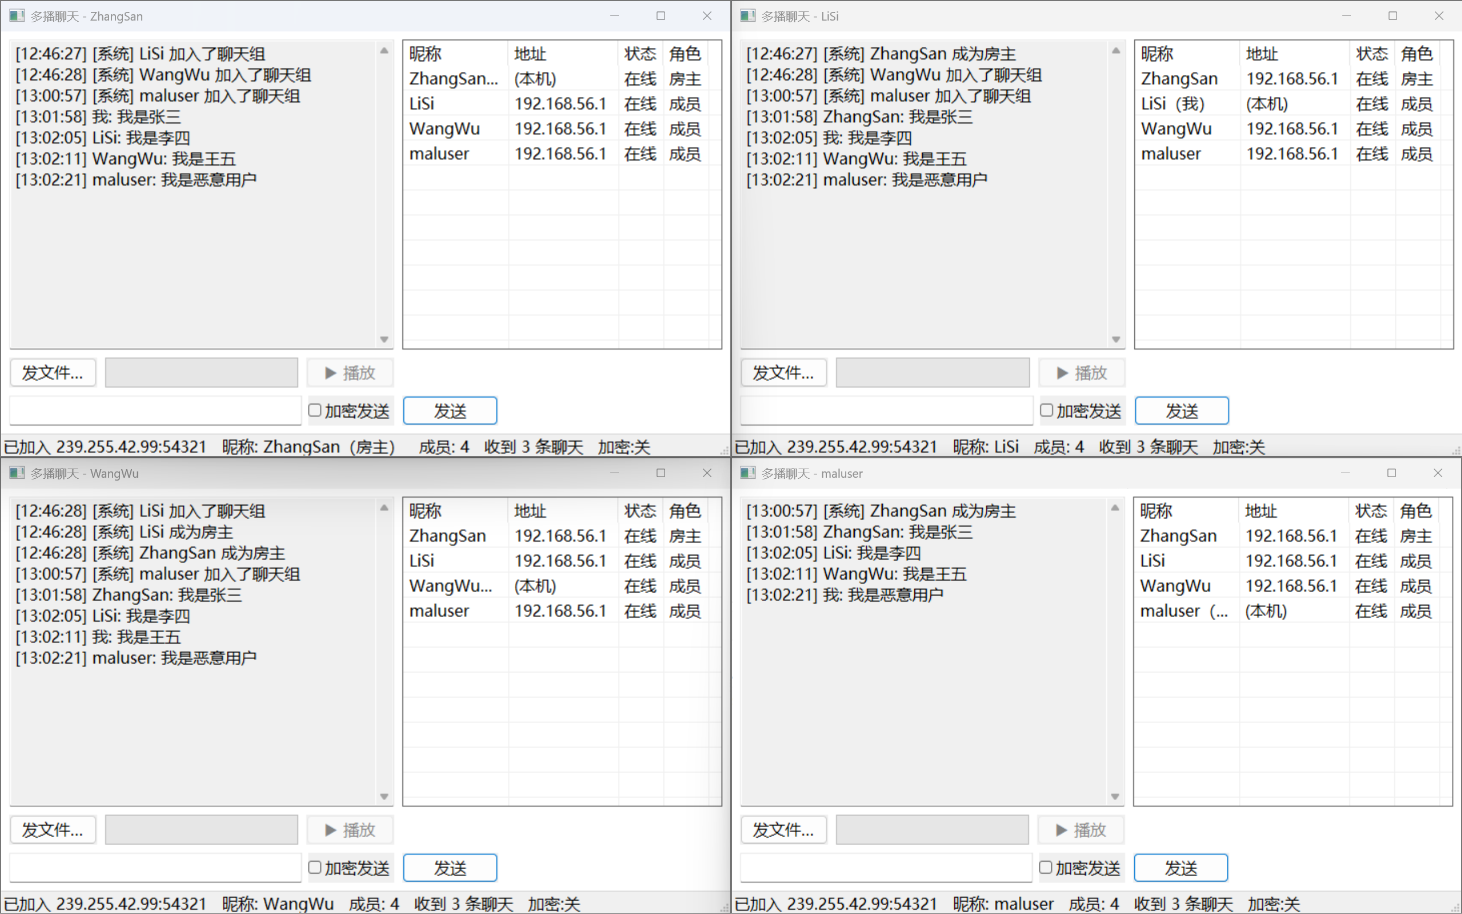
\includegraphics[width=0.98\textwidth]{figures/fig_members.png}
\caption{四实例跨机聊天：成员列表一致，恶意用户 maluser 入组}
\label{fig:members}
\end{figure}

图~\ref{fig:kick} 是房主 ZhangSan 踢出 maluser 的瞬间：maluser 端收到
"你已被房主 ZhangSan 移出聊天组，3 秒后自动退出"，输入框与发送按钮被禁用，
成员数回落为 3；其余成员同步把 maluser 从列表删除并加入黑名单——其后续报文
（即使伪造）一律被忽略。

\begin{figure}[H]
\centering
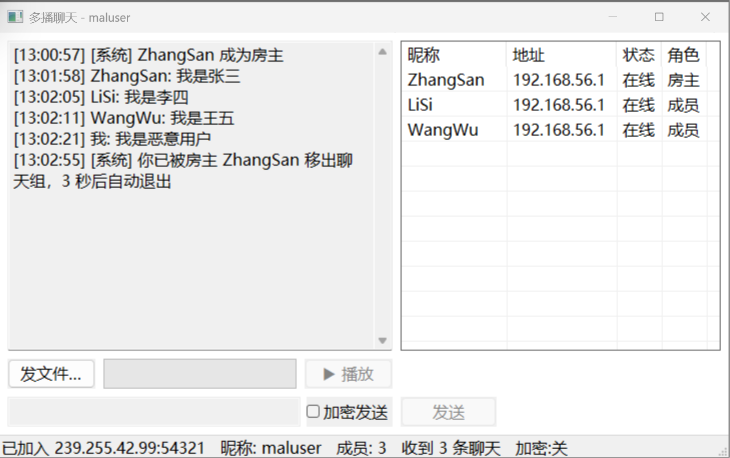
\includegraphics[width=0.42\textwidth]{figures/fig_kick.png}
\caption{房主踢出 maluser：被踢端收到签名验证通过的 KICK 后禁用输入并自动退出}
\label{fig:kick}
\end{figure}

\subsection{单机部署与跨机部署的对比}

本系统的验证同时覆盖了单机多实例（回环）与跨机（VirtualBox Host-Only 网段
192.168.56.0/24，宿主机与虚拟机同网段）两种部署。两者的\textbf{协议行为完全一致}
——实例间零共享状态、纯报文同步，应用层无法区分报文来源——差别只在网络路径本身：

\begin{table}[H]
\centering\footnotesize
\begin{tabularx}{0.98\textwidth}{lXX}
\toprule
 & 单机多实例（回环） & 跨机（同一局域网） \\
\midrule
网络路径 & 内核回环，不出网卡 & 真实以太网帧（多播 MAC） \\
丢包率 & 接近 0（缓冲充足时） & 真实网络拥塞/缓冲溢出都会发生 \\
IGMP/交换机依赖 & 无 & 需要 AP/交换机放行多播（部分 WiFi 屏蔽） \\
验证重点 & 功能正确性 & 真实丢包下的可靠性（NACK） \\
\bottomrule
\end{tabularx}
\caption{两种部署方式的差异：协议层一致，网络路径不同}
\label{tab:deploy}
\end{table}

\noindent 正因回环路径几乎不丢包，可靠性机制在单机上"看不出来"，所以除真实跨机
传输外，代码内置 \texttt{-{}-drop N} 钩子在接收端人为丢弃每第 $N$ 块，使单机也能
复现高丢包场景（\S\ref{sec:auto} 中 20\% 丢块的用例即来源于此）。

\subsection{文件传输与播放（要求 b）}

图~\ref{fig:file} 中 ZhangSan 依次发送 ACPN-HW01.ppt 与 VID\_20261031\_130401.mp4，
LiSi 与 WangWu 两端同时显示"开始接收（来自 ZhangSan）"与"接收完成"，文件经
SHA-256 校验后保存在 exe 目录的 \texttt{received\textbackslash} 下；接收端点"播放"
由系统媒体播放器直接打开视频（右下角）。注意接收端文件名自动变为
"ACNP-HW01 (1).ppt"——同名冲突时的唯一化命名生效。一次多播、两个接收方各自独立
收全，1-N 语义成立。

\begin{figure}[H]
\centering
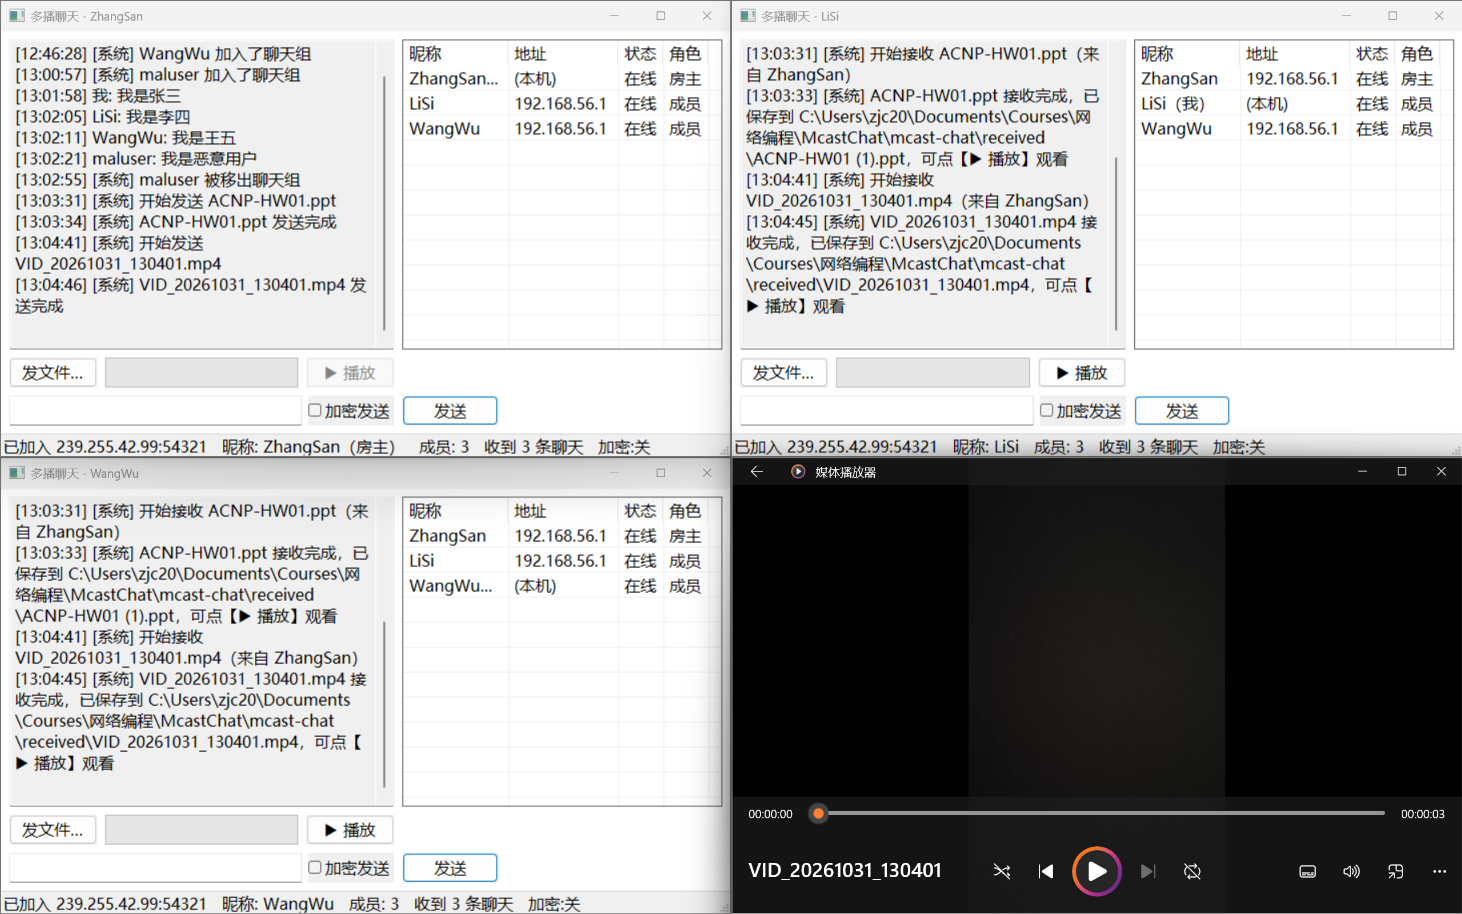
\includegraphics[width=0.95\textwidth]{figures/fig_file.png}
\caption{多播文件传输：ppt 与 mp4 同时发往两台接收方，右下为接收端播放视频}
\label{fig:file}
\end{figure}

\subsection{加密传输验证（要求 d）}

图~\ref{fig:crypto} 是 tshark 在多播出接口抓到的真实报文（自动化流程：B 先在
加密关闭时发送明文文本，随后房主开启加密并分发组密钥，B 再发同一类文本）。
上方面包明文可见：载荷里 utf8 编码的昵称与正文（\texttt{LiSi}、
\texttt{hello-plaintext-12345}）在 ASCII 列直接可读；下方开启加密后同为 TEXT
报文，flags 变为 0x0003（ENCRYPTED|SIGNED），载荷变成 keyId + 随机分布的密文。
对整个抓包文件检索两个标记串的 UTF-8 字节：\textbf{密文报文中 0 次命中}。

本次抓包共 25 个 MCHT 报文，构成如下：明文/密文 TEXT 各 1 个、KEY\_DIST 信封分发
报文 2 个（房主开关加密与成员加入各触发一次换钥），其余为 HELLO/HEARTBEAT/ACK
等控制报文。两个 TEXT 报文的载荷对比很能说明信封方案的带宽代价：明文 285\,B
（正文 29\,B + 签名 256\,B），密文 302\,B（keyId 4\,B + 密文 42\,B + tag 16\,B +
签名 256\,B）——加密本身只增加了 20 字节，签名的占比反而更大，这正是"非对称算法
只签小数据、Bulk 数据交给对称算法"的直接体现。

\begin{figure}[H]
\centering
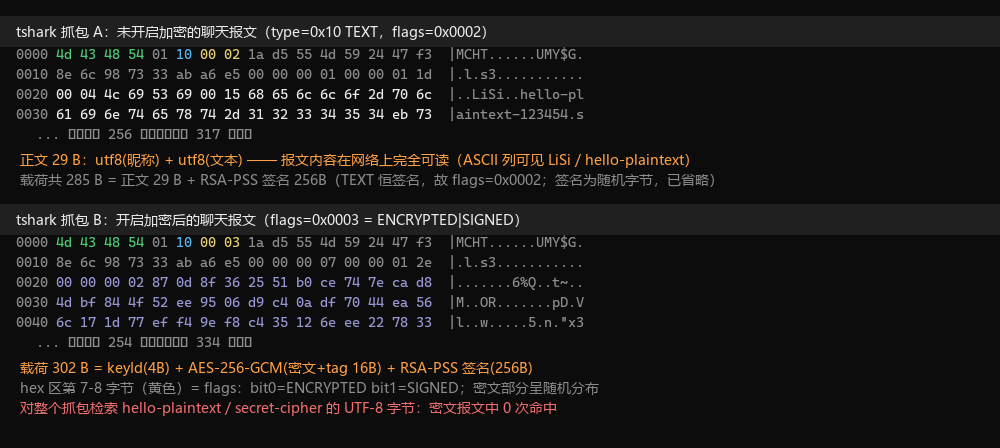
\includegraphics[width=0.88\textwidth]{figures/fig_crypto.png}
\caption{tshark 抓包对比：加密前的明文载荷与加密后的密文载荷（真实抓包数据）}
\label{fig:crypto}
\end{figure}

\subsection{自动化测试}
\label{sec:auto}

为避免手工回归，配套 8 阶段自动化冒烟测试（PowerShell 驱动真实多实例，通过
WM\_GETTEXT/WM\_SETTEXT 读写控件断言），29 项检查全部通过，覆盖：单机多实例
互聊、BYE 离开、房主踢人、心跳超时（10\,s 离线/20\,s 移除）、文件传输、加密端到端。
其中文件传输用例在接收端开启 \texttt{-{}-drop 5}（人为丢弃约 20\% 的块）：
2\,MB 随机文件首轮缺失 \textbf{410 块，仅 1 轮 NACK 重传即收全，SHA-256 与源文件一致}。
另有独立网络自测 \texttt{nettest}：同机两个多播套接字各收到全部 10/10 个探测包，
验证了"多播回环 + 端口复用"下单机多实例的可达性。

\begin{table}[H]
\centering\footnotesize
\begin{tabularx}{0.98\textwidth}{p{0.6cm}Xl}
\toprule
编号 & 用例 & 结果 \\
\midrule
1 & 编译（\texttt{-O2 -Wall -Wextra}） & 零警告，单命令 \texttt{build.bat} 出静态链接 exe \\
2 & 单机 3 实例文字聊天 & 一次发送，其余实例同步收到（多播回环） \\
3 & 跨机 4 实例（VirtualBox Host-Only） & 成员列表四处一致，含 IP 与角色 \\
4 & 心跳保活 & 强杀进程后 10\,s 标记离线、20\,s 自动移除 \\
5 & BYE 退出 & 关闭窗口即多播 BYE，对端立即移除 \\
6 & 房主踢人 & 被踢端禁用输入、3\,s 自动退出；黑名单生效 \\
7 & 房主离线 & 自动由 joinTime 次早者继任 \\
8 & 2\,MB 文件 + 20\% 人为丢块 & 缺失 410 块，1 轮 NACK 收全，SHA-256 一致 \\
9 & 加密文本 & 房主分发密钥后，对端解密显示正确 \\
10 & 加密文件（叠加 20\% 丢块） & 收全且 SHA-256 一致 \\
11 & 抓包检索 & 密文报文中明文标记串 0 次命中 \\
12 & 接收路径锚定 & 实例工作目录设在桌面，文件仍落 exe 目录 \\
13 & \texttt{nettest} 多播自测 & 同机双套接字各收全 10/10 个探测包 \\
14 & TEXT 签名 & 未开启加密时 flags=0x0002（仅签名），验签通过才显示 \\
15 & 密钥分发抓包 & 捕获 2 个 KEY\_DIST 报文（开关加密、成员加入各触发一次） \\
16 & 重名唯一化 & 再次接收同名文件自动存为"原名 (1).ext" \\
17 & 20\% 丢块下加密文件 & 512\,KB 随机文件叠加 \texttt{-{}-drop 5}，收全且 SHA-256 一致 \\
\bottomrule
\end{tabularx}
\caption{主要测试用例与结果（完整 29 项见仓库 \texttt{test/smoke.ps1}）}
\label{tab:cases}
\end{table}

\section{交付物与复现方法}

\begin{lstlisting}[caption={交付物与一键复现}]
McastChat/                  仓库根（源码 + 报告 tex/pdf + 测试）
 |- mcast-chat/             源码工程：src/ + build.bat + demo.bat（零第三方依赖）
 |- report/report.tex       本报告源文件（XeLaTeX，bash build.sh 编译）
 |- report/report.pdf       编译产物
 |- ARCHITECTURE.md         设计文档（架构/协议/各阶段实现备注）
 |- MANUAL.md               操作手册
 |- test/smoke.ps1          8 阶段自动化测试（29 项检查）
 `- test/nettest.cpp        多播可达性自测
\end{lstlisting}

\noindent 复现：运行 \texttt{mcast-chat\textbackslash build.bat} 编译；双击
\texttt{demo.bat} 或 \texttt{mcast-chat.exe 昵称} 启动；勾选"加密发送"体验加密；
\texttt{test/smoke.ps1} 重跑全部自动化验证；\texttt{report/build.sh} 重编译本报告。

\section{实验总结}

本作业用约 4600 行 C++ 实现了一个完全去中心化的多播聊天工具：文字聊天、可靠文件
传输、成员管理与非对称加密全部构建在一个 UDP 多播组之上，无任何服务器参与。

对多播的理解是最大的收获。多播的组成员关系在 IP/IGMP 层，应用层查不到，所以
"显示成员、踢出成员"必须靠应用层握手与心跳自建成员表；而多播本身不提供可靠性，
2\,MB 文件丢 20\% 的块仍能靠一轮 NACK 区间重传收全，说明"节拍发送 + 接收位图 +
区间化 NACK"这套组合对不可靠信道是够用的。单机演示的原理也值得记录：
\texttt{IP\_MULTICAST\_LOOP} 让内核把多播包回送本机，\texttt{SO\_REUSEADDR} 让多个
实例共存于同一端口，内核按组成员关系逐套接字投递副本——由于实例间零共享状态、
纯报文同步，单机验证与跨机部署的协议行为完全一致，实测跨虚拟机（192.168.56.x）
结果与单机相同。

加密部分的结论是"信封"而非"全用 RSA"：RSA-2048 只加密 32\,B 的组密钥，实际载荷
由 AES-256-GCM 保护，nonce 从 senderId 与 seq 确定性派生、AAD 绑定包头，既省带宽
又防重放与拼接；换钥时保留上一把密钥按 keyId 回退，使密钥轮换不打断正在进行的
文件传输，被踢者则因拿不到新密钥被应用层强制隔离。tshark 抓包对比直观展示了
加密前后载荷的差异，也验证了签名的存在（flags 恒为 0x0002/0x0003）。

工程上踩掉的四个坑都很有代表性：Windows 头文件里 \texttt{FILE\_END} 宏与自定义
枚举撞名；只读编辑控件会拦截 \texttt{EM\_REPLACESEL}（追加文本前须临时解除只读）；
跨进程 \texttt{GetWindowText} 读到的是系统缓存的标题而非控件真实内容（自动化测试
必须改用 \texttt{WM\_GETTEXT}）；文件对话框会改变进程工作目录，落盘路径必须用
绝对路径锚定。它们共同指向同一条经验：\textbf{平台 API 的隐式行为必须实测，不能
想当然}。

\begin{thebibliography}{9}
\bibitem{xie} 谢希仁. 计算机网络（第 8 版）. 电子工业出版社, 2021.（第 4 章：网络层与 IP 多播）
\bibitem{stevens} W. Richard Stevens. TCP/IP Illustrated, Vol.~1: The Protocols (2nd ed.). Addison-Wesley, 2011.（第 13--15 章：广播与多播、IGMP）
\bibitem{rfc1112} S. Deering. Host Extensions for IP Multicasting. RFC 1112, 1989.
\bibitem{rfc5740} B. Adamson et al. NACK-Oriented Reliable Multicast (NORM) Protocol. RFC 5740, 2009.（本作业 NACK 区间重传的简化原型）
\bibitem{msdn} Microsoft Learn. Winsock Reference; CNG (bcrypt.h) API. \url{https://learn.microsoft.com/windows/win32/}
\end{thebibliography}

\end{document}
